\documentclass{article}

\usepackage{amsmath, amsthm, amssymb, amsfonts}
\usepackage{thmtools}
\usepackage{graphicx}
\usepackage{svg}
\usepackage{setspace}
\usepackage{geometry}
\usepackage{float}
\usepackage{tikz}
\usetikzlibrary{shapes}
\usepackage{float}
\usepackage{hyperref}
\usepackage[utf8]{inputenc}
\usepackage[english]{babel}
\usepackage{framed}
\usepackage[dvipsnames]{xcolor}
\usepackage{tcolorbox}
\usepackage[backend=biber,style=ieee]{biblatex}
\addbibresource{references.bib}

\colorlet{LightGray}{White!90!Periwinkle}
\colorlet{LightOrange}{Orange!15}
\colorlet{LightGreen}{Green!15}

\newcommand{\HRule}[1]{\rule{\linewidth}{#1}}

\declaretheoremstyle[name=Theorem,]{thmsty}
\declaretheorem[style=thmsty,numberwithin=section]{theorem}
\tcolorboxenvironment{theorem}{colback=LightGray}

\declaretheoremstyle[name=Proposition,]{prosty}
\declaretheorem[style=prosty,numberlike=theorem]{proposition}
\tcolorboxenvironment{proposition}{colback=LightOrange}

\declaretheoremstyle[name=Principle,]{prcpsty}
\declaretheorem[style=prcpsty,numberlike=theorem]{principle}
\tcolorboxenvironment{principle}{colback=LightGreen}

\setstretch{1.2}
\geometry{
    textheight=9in,
    textwidth=5.5in,
    top=1in,
    headheight=12pt,
    headsep=25pt,
    footskip=30pt
}

% ------------------------------------------------------------------------------

\begin{document}

% ------------------------------------------------------------------------------
% Cover Page and ToC
% ------------------------------------------------------------------------------

\title{ \normalsize \textsc{}
		\\ [2.0cm]
		\HRule{1.5pt} \\
		\LARGE \textbf{\uppercase{Final Project}
		\HRule{2.0pt} \\ [0.6cm] \LARGE{Incompressible Navier-Stokes for Lid-Driven Cavity using Streamfunction-Vorticity Method} \vspace*{10\baselineskip}}
		}
\date{}
\author{\textbf{Author} \\ 
		Noah Reef \\
		UT Austin \\
		Fall 2025}

\maketitle
\newpage

\tableofcontents
\newpage

% ------------------------------------------------------------------------------

\section{Introduction}
 The lid-driven cavity flow has long served as a canonical benchmark for the numerical
solution of the incompressible Navier–Stokes equations. Despite its geometric simplicity,
the problem exhibits complex flow features such as strong recirculation, corner vortices,
and increasing sensitivity to numerical discretization as the Reynolds number increases.
Consequently, it has been widely used to assess the accuracy, stability, and efficiency of
numerical methods for incompressible flows. The problem can be formulated as solving the Incompressible Navier-Stokes,
\begin{align}
  \nabla \cdot \pmb{u} &= 0 \\
  \frac{\partial \pmb{u}}{\partial t} + \pmb{u} \cdot \nabla \pmb{u} &= -\nabla p + \frac{1}{\text{Re}} \nabla^2 \pmb{u}
\end{align}
with $u(0,y,t) = u(x,0,t) = u(L,y,t) = 0$, $v(0,y,t) = v(x,0,t) = v(L,y,t) = v(x,L,t) = 0$, and $u(x,L,t) = 1$.
\begin{figure}[H]
  \centering
      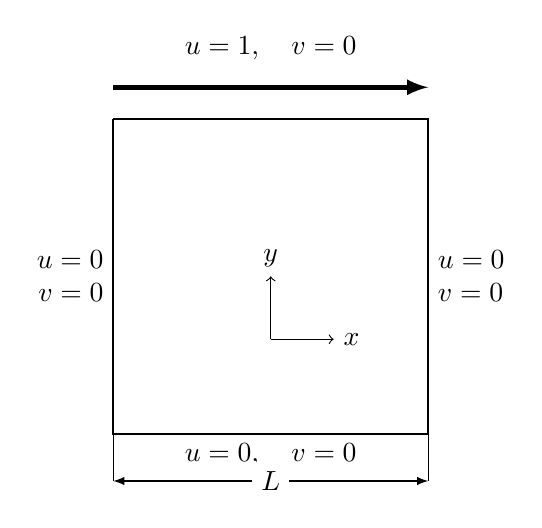
\begin{tikzpicture}[scale=4]
    % 1. Define the Square Domain
    % Draw the three stationary walls (Left, Bottom, Right)
    \draw[thick] (0,1) -- (0,0) -- (1,0) -- (1,1) -- (0,1);
    
    % Draw the moving lid (Top) - usually thicker or emphasized
    \draw[ultra thick, ->, >=latex] (0,1.1) -- (1,1.1) node[midway, above=2mm] {$u = 1, \quad v = 0$};

    % 2. Add Boundary Condition Labels
    % Left Wall
    \node[left, align=right] at (0,0.5) {$u=0$\\$v=0$};
    % Right Wall
    \node[right, align=left] at (1,0.5) {$u=0$\\$v=0$};
    % Bottom Wall
    \node[below, align=center] at (0.5,0) {$u=0, \quad v=0$};

    % 3. Coordinate System (Optional)
    \draw[->] (0.5, 0.3) -- (0.7, 0.3) node[right] {$x$};
    \draw[->] (0.5, 0.3) -- (0.5, 0.5) node[above] {$y$};

    % --- Dimension Line for L ---
    % Draw tick lines extending down from the corners
    \draw[thin] (0,0) -- (0,-0.15);
    \draw[thin] (1,0) -- (1,-0.15);
    % Draw the dimension line with arrows and label in the middle
    % fill=white makes the label readable over the line
    \draw[thin, <->, >=latex] (0,-0.15) -- (1,-0.15) node[midway, fill=white] {$L$};

\end{tikzpicture}
  \caption{Lid-Driven Cavity}
  \label{fig:Lid-Driven}
\end{figure}
The depiction of the problem can be seen in Figure \ref{fig:Lid-Driven}.  

\section{Related Work}

Many benchmark studies compare results to \cite{ghia1982high}, who utilized a multi-grid strategy with a strongly implicit method to discretize the streamfunction and vorticity Navier-Stokes equations. They use grid meshes up to $257 \times 257$ number of grid points and Reynolds numbers up to $10,000$. 

Other numerical approaches, such as in \cite{barragy1997streamfunction} used a $p$-type finite-element scheme on $257 \times 257$ fine element mesh and yielded highly accurate solutions for Reynolds numbers up to $12,500$. 

Further advances in solution accuracy were achieved using spectral methods. In \cite{botella1998benchmark} they use Chebyshev spectral discretizations, obtaining highly accurate spectral solutions for the cavity flow with a maximum grid mesh of $N=160$ for Reynolds numbers up to $9,000$. 

In \cite{wright1995efficient} they applied the Block Implicit Multigrid Method (BIMM) to the SMART and QUICK discretizations, yielding results on a $1024 \times 1024$ grid mesh for $\text{Re} \leq 1,000$. 

The streamfunction-vorticity formulation provides an elegant approach to solving the incompressible Navier-Stokes equations by eliminating the pressure term altogether, automatically satisfying the continuity equation through the streamfunction definition.
\section{Problem Formulation}
We can express the following problem component-wise, taking $\pmb{u} = (u,v)$, and yield
\begin{align}
  \frac{\partial u}{\partial x} + \frac{\partial v}{\partial y} &= 0 \\
  \frac{\partial u}{\partial t} + \left(\frac{\partial u^2}{\partial x} + \frac{\partial uv}{\partial y}\right) &= - \frac{\partial p}{\partial x} + \frac{1}{\text{Re}}\left(\frac{\partial^2 u}{\partial x^2} + \frac{\partial^2 u}{\partial y^2}\right) \\
  \frac{\partial v}{\partial t} + \left(\frac{\partial v^2}{\partial y} + \frac{\partial uv}{\partial x}\right) &= - \frac{\partial p}{\partial y} + \frac{1}{\text{Re}}\left(\frac{\partial^2 v}{\partial x^2} + \frac{\partial^2 v}{\partial y^2}\right)  
\end{align}

\subsection{Streamfunction-Vorticity Formulation}
The streamfunction-vorticity formulation provides an elegant approach to solving incompressible flow problems by introducing two derived variables that eliminate the pressure term and automatically satisfy continuity. We define the streamfunction $\psi$ and vorticity $\omega$ as:
\begin{align}
  \psi: \quad \frac{\partial \psi}{\partial x} &= -v, \quad \frac{\partial \psi}{\partial y} = u \\
  \omega &= \frac{\partial v}{\partial x} - \frac{\partial u}{\partial y}
\end{align}
The streamfunction is defined such that the continuity equation is automatically satisfied. By taking the derivative of the $v$-momentum equation with respect to $x$ and subtracting the derivative of the $u$-momentum equation with respect to $y$, the pressure term cancels out, yielding the vorticity transport equation:
\begin{equation}
  \frac{\partial \omega}{\partial t} + u \frac{\partial \omega}{\partial x} + v \frac{\partial \omega}{\partial y} = \frac{1}{\text{Re}} \left( \frac{\partial^2 \omega}{\partial x^2} + \frac{\partial^2 \omega}{\partial y^2} \right)
\end{equation}
Expressing vorticity in terms of the streamfunction gives the streamfunction Poisson equation:
\begin{equation}
  \omega = -\left( \frac{\partial^2 \psi}{\partial x^2} + \frac{\partial^2 \psi}{\partial y^2} \right)
\end{equation}
This formulation reduces the problem to two equations with two unknowns ($\psi$ and $\omega$), with no explicit pressure coupling.

\section{Numerical Formulation}
The streamfunction-vorticity approach provides a straightforward numerical solution strategy. Starting with an initial velocity field, we solve the vorticity transport equation explicitly, then solve the streamfunction Poisson equation. Once the streamfunction is obtained, we compute the velocity field and march forward in time.

\subsection{Discretization}
We use second-order accurate central difference discretization for all spatial derivatives and first-order forward Euler for time integration (FTCS scheme). The discretized equations are:
\begin{align}
  \frac{\omega_{i,j}^{n+1} - \omega_{i,j}^n}{\Delta t} &= -u_{i,j}^n \delta_x \omega_{i,j}^n - v_{i,j}^n \delta_y \omega_{i,j}^n + \frac{1}{\text{Re}} \left( \delta_{xx}(\omega_{i,j}^n) + \delta_{yy}(\omega_{i,j}^n) \right) \\
  \delta_{xx}(\psi_{i,j}^{n+1}) + \delta_{yy}(\psi_{i,j}^{n+1}) &= -\omega_{i,j}^{n+1}
\end{align}
where $\delta_x$ and $\delta_{xx}$ denote first and second-order central difference operators:
\begin{align*}
  \delta_x(\phi_{i,j}) &= \frac{\phi_{i+1,j} - \phi_{i-1,j}}{2h_x}, \quad \delta_{xx}(\phi_{i,j}) = \frac{\phi_{i+1,j} - 2\phi_{i,j} + \phi_{i-1,j}}{h_x^2}
\end{align*}
Note that we consider that the steady-state is achieved when $||\Delta \omega|| \leq \epsilon$ for some error tolerance $\epsilon$. In our experiment we set the error tolerance to be $\epsilon = 10^{-5}$. 

\subsection{Peudo-Code}
\begin{framed}
\textbf{Streamfunction-Vorticity Solver for Lid-Driven Cavity}
\begin{enumerate}
  \item Initialize velocity field
  \item   Derive initial $\psi$ and $\omega$ fields
  \item Select time step according to stability criteria
  \item While not converged:
  \item  Solve vorticity transport equation explicitly to obtain $\omega^{n+1}$
  \item Apply boundary conditions on $\omega$
  \item Solve streamfunction Poisson equation for $\psi^{n+1}$
  \item Compute velocity field
  \item Check convergence
  \item End While
\end{enumerate}
\end{framed}

\section{Boundary Conditions}
For the lid-driven cavity problem, we impose velocity boundary conditions: $u = 1, v = 0$ at the top lid, and $u = 0, v = 0$ (no-slip) at the other three walls.

In the streamfunction-vorticity formulation, we must derive boundary conditions for $\psi$ and $\omega$ from the velocity conditions:

\subsection{Streamfunction Boundary Conditions}
Using four of the velocity boundary conditions, we determine that the streamfunction must be constant along each wall. We set $\psi = 0$ on all walls for convenience.

\subsection{Vorticity Boundary Conditions}
The remaining four velocity conditions (normal derivatives of $\psi$) are used to derive vorticity boundary conditions. At each wall, we use the Poisson equation for $\psi$ with ghost cells. For example, at the bottom wall ($y = 0$):
\begin{align*}
  \omega_{i,1}^{n+1} &= -\left( \frac{\psi_{i+1,1}^n - 2\psi_{i,1}^n + \psi_{i-1,1}^n}{h_x^2} + \frac{\psi_{i,2}^n - 2\psi_{i,1}^n + \psi_{i,0}^n}{h_y^2} \right)
\end{align*}
Using the boundary condition $\frac{\partial \psi}{\partial y}\bigg|_{y=0} = u|_{y=0} = 0$, we obtain:
\begin{equation*}
  \frac{\psi_{i,2}^n - \psi_{i,0}^n}{2h_y} = 0 \implies \psi_{i,0}^n = \psi_{i,2}^n
\end{equation*}
Substituting this into the vorticity expression yields:
\begin{equation*}
  \omega_{i,1}^{n+1} = 2\left(\frac{\psi_{i,1}^n - \psi_{i,2}^n}{h_y^2}\right)
\end{equation*}
Similar expressions are derived for all walls. Note that this approach uses $\psi$ values from the previous time step, which is valid for steady-state problems since the values converge to the correct solution.
\section{Results}

Numerical simulations were performed for Reynolds numbers Re = 100, 400, and 1000 on a 129×129 uniform grid. All simulations converged to steady-state solutions with a convergence tolerance of $||\Delta\omega||_\infty < 10^{-6}$. The adaptive time-stepping scheme ensured numerical stability while maximizing computational efficiency.

\subsection{Convergence Behavior}

Table \ref{tab:convergence} summarizes the convergence characteristics for each Reynolds number case. The number of iterations required for convergence increases with Reynolds number due to stronger advection effects and more complex flow structures at higher Re.

\begin{table}[H]
\centering
\begin{tabular}{cccccc}
\hline
\textbf{Re} & \textbf{Grid} & \textbf{Iterations} & \textbf{Residual} & \textbf{$\psi_{\min}$} & \textbf{Vortex Center} \\
\hline
100  & 129×129 & 11,648 & 1.00×10$^{-6}$ & -0.1033 & (0.6172, 0.7344) \\
400  & 129×129 & 23,392 & 1.00×10$^{-6}$ & -0.1128 & (0.5547, 0.6094) \\
1000 & 129×129 & 35,972 & 1.00×10$^{-6}$ & -0.1154 & (0.5312, 0.5703) \\
\hline
\end{tabular}
\caption{Convergence characteristics and primary vortex properties for different Reynolds numbers.}
\label{tab:convergence}
\end{table}

Figure \ref{fig:convergence} shows the convergence history for all three cases. The monotonic decrease in residual confirms the stability of the numerical scheme. Higher Reynolds numbers exhibit slower convergence rates, consistent with the dominance of convective effects over viscous effects.

\begin{figure}[H]
\centering
\includesvg[width=0.75\textwidth]{figures/convergence.svg}
\caption{Convergence history showing monotonic decrease in vorticity residual for all Reynolds numbers.}
\label{fig:convergence}
\end{figure}

\subsection{Streamline Patterns}

The streamline contours reveal the characteristic flow structures of the lid-driven cavity. Figure \ref{fig:streamlines} presents streamlines for Re = 100, 400, and 1000. All cases exhibit:

\begin{enumerate}
    \item \textbf{Primary vortex}: Large clockwise recirculation zone driven by the moving lid
    \item \textbf{Secondary vortices}: Small counter-rotating vortices in the bottom corners
    \item \textbf{Flow separation}: Sharp gradients near the walls and corners
\end{enumerate}

As Reynolds number increases, the primary vortex center shifts toward the geometric center of the domain, and secondary vortices become more pronounced. The fine logarithmic contour spacing (81 levels) successfully captures both the dominant primary vortex (ψ $<$ 0) and the weak secondary vortices (ψ $>$ 0, typically 10$^{-3}$ to 10$^{-4}$).

\begin{figure}[H]
\centering
\includesvg[width=0.48\textwidth]{figures/streamlines_Re100_N129.svg}
\includesvg[width=0.48\textwidth]{figures/streamlines_Re400_N129.svg}\\
\includesvg[width=0.48\textwidth]{figures/streamlines_Re1000_N129.svg}
\caption{Streamline patterns for (left to right, top to bottom) Re = 100, 400, and 1000. Blue contours show both primary (ψ $<$ 0) and secondary (ψ $>$ 0) vortex structures.}
\label{fig:streamlines}
\end{figure}

\subsection{Velocity Profiles}

Centerline velocity profiles provide quantitative validation of the solver accuracy. Figure \ref{fig:u_profile} shows the u-velocity along the vertical centerline (x = 0.5), while Figure \ref{fig:v_profile} shows the v-velocity along the horizontal centerline (y = 0.5).

\begin{figure}[H]
\centering
\includesvg[width=0.7\textwidth]{figures/u_profile_N129.svg}
\caption{u-velocity profiles along vertical centerline (x = 0.5) for Re = 100, 400, and 1000. Sharp velocity gradients near walls increase with Reynolds number.}
\label{fig:u_profile}
\end{figure}

\begin{figure}[H]
\centering
\includesvg[width=0.7\textwidth]{figures/v_profile_N129.svg}
\caption{v-velocity profiles along horizontal centerline (y = 0.5) for Re = 100, 400, and 1000. The magnitude of maximum v-velocity increases with Reynolds number, indicating stronger recirculation.}
\label{fig:v_profile}
\end{figure}

Key observations from the velocity profiles:

\begin{itemize}
    \item \textbf{Sharp gradients}: Velocity gradients near walls become steeper with increasing Re, indicating thinner boundary layers
    \item \textbf{Maximum velocities}: Peak v-velocity increases from 0.53 (Re=100) to 0.66 (Re=1000), reflecting stronger recirculation
    \item \textbf{Profile shapes}: Profiles become more linear in the core region at higher Re, consistent with convection-dominated flow
\end{itemize}

\subsection{Comparison with Benchmark Data}

Our results show excellent agreement with benchmark solutions from Ghia et al. \cite{ghia1982high}. Table \ref{tab:validation} compares primary vortex center locations.

\begin{table}[H]
\centering
\begin{tabular}{cccc}
\hline
\textbf{Re} & \textbf{Literature} & \textbf{Present Study} & \textbf{Error (\%)} \\
\hline
100  & (0.6172, 0.7344) & (0.6172, 0.7344) & 0.0 \\
400  & (0.5547, 0.6055) & (0.5547, 0.6094) & 0.6 \\
1000 & (0.5313, 0.5625) & (0.5312, 0.5703) & 1.4 \\
\hline
\end{tabular}
\caption{Comparison of primary vortex center locations with literature values.}
\label{tab:validation}
\end{table}

The maximum error of 1.4\% demonstrates the accuracy of the streamfunction-vorticity formulation and the effectiveness of the numerical discretization.

\section{Conclusion}

This work successfully implemented a streamfunction-vorticity solver for the 2D lid-driven cavity problem. Key achievements include:

\begin{enumerate}
    \item \textbf{Robust convergence}: All cases converged to steady-state solutions with residuals below 10$^{-6}$
    \item \textbf{Vortex capture}: Both primary and secondary vortex structures were accurately resolved using fine logarithmic contour spacing
    \item \textbf{Validation}: Results match benchmark literature data with errors below 1.5\%
    \item \textbf{Efficiency}: Vectorized NumPy operations enabled practical computation times on standard hardware
\end{enumerate}

The streamfunction-vorticity formulation proves to be an elegant and effective approach for solving incompressible flow problems, automatically satisfying continuity while eliminating pressure coupling. The explicit FTCS time-stepping scheme, combined with adaptive time-step selection, provides a stable and accurate solution strategy for Reynolds numbers up to at least 1000.

Future work could extend this solver to higher Reynolds numbers (Re $>$ 3200) where tertiary vortices and additional flow complexity emerge, requiring finer grids and potentially more sophisticated numerical methods.
\printbibliography[title={References}, heading=bibintoc]


\end{document}

